\chapter{Preliminaries}
\label{chap:Preliminaries}

In this section, the streaming data and the model basic will be introduced. At first, we formally define the data stream used in the experiments. Furthermore, we figure out the definition of anomalies in streaming data, and metrics used for evaluation. Finally we refer the main concept of autoencoders and LSTMs, which are the basic architecting and component of our model. Table 3.1 is a summarization of notations used in this section.

\begin{table}[h]
\begin{center}
\begin{tabular}{|l|l|}
\hline
Notation & Description \\ \hline
DS & Data stream \\
$x_i$ & Instance arrived at moment i \\
$t_i$ & Timestamp of moment i \\
MB & Batch size	\\	
T & LSTM unit input window length \\
$c \in R^{hs}$ & LSTM unit cell state with hs dimensions \\
$a \in R^{T}$ & Cell output with T dimensions \\ 
$\chi = R^d $ & Feature space with d dimensions  \\
X & A random variable take values from $\chi$	\\
$\Phi$ & Shaping function of autoencoders	\\	
$\Psi$ & Activation function of autoencoders	 \\
H & Hidden layer representation of autoencoders  \\
$d_j$ & Decoder input at step j\\ \hline

\end{tabular}
\end{center}
\label{tab:notation}
\caption{Table of notations}
\end{table}


\section{Definition of stream}
\label{sec:Definition of stream}

Assume that a set of devices or data warehouses generate data continuously (here we only take about numerical data). A data stream DS is defined as 
\begin{equation} \label{eq:DS}
DS = \{(x_1,t_1),(x_2,t_2), ... , (x_T,t_T), ...\}
\end{equation}
where \textbf{$x_T$} is the instance arrived at timestamp \textbf{$t_T$} and represented by a multi-dimensional vector.\\

In order to feed the streaming data to LSTMs, the stream is accumulated to windows and batches as \Fref{fig:stream}. Every T instances are accumulated to a window as a single LSTM input. And MB is the predefine batch size, each batch contains MB windows.\\

\begin{figure}[h]
\centering
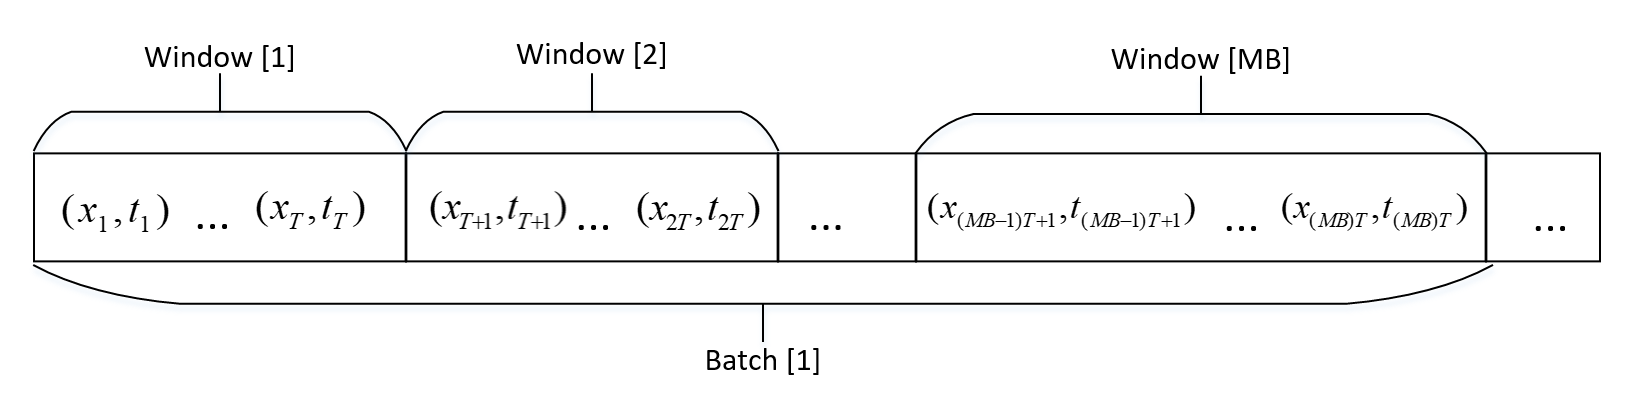
\includegraphics[width=12cm, height=3cm]{stream}
\caption[Data stream]{Data stream}
\label{fig:stream}
\end{figure}




\section{Definition of anomalies}
\label{sec:Definition of anomalies}

\textbf{Pointwise}: A data point (instance) is anomalous(e.g. \Fref{fig:point}) if this point is distant from other observations according to some specific measurement metrics. This is used in fine-grained anomaly detection tasks, that need to find out every single anomalous instance, e.g. credit card fraud detection, spam email detection.\\

\textbf{Window-based}: Sometimes, a data point is apparently normal, but this point, or potentially together with its neighbors violates the overall periodicity or other character of the time series, we also treat them as anomaly, which is called window-based anomaly or contextual anomaly, e.g. \Fref{fig:window}.\\


In the anomlay detection experiments, abnormal data is the object of study, therefore we take the anomaly as positive class and normal data as negative class. \\

\begin{table}[h]
\begin{center}
\begin{tabular}{l|l|c|c|}
\multicolumn{2}{c}{}&\multicolumn{2}{c}{Actual value}\\
\cline{3-4}
\multicolumn{2}{c|}{}&Normal&Abnormal\\
\cline{2-4}
\multirow{2}{*}{Prediction}& Normal & $TN$ & $FN$\\
\cline{2-4}
& Abnormal & $FP$ & $TP$\\
\cline{2-4}
\end{tabular}
\end{center}
\label{tab:conf}
\caption{Confusion matrix}
\end{table}

The target is to achieve higher true positive rate (equation \ref{eq:tpr}, true alarms) while remain lower false positive rate (equation \ref{eq:fpr}, wrong alarms). The evaluation metric is Area Under the Curve (AUC), where the curve is receiver operating characteristic curve, and is created by plotting the true positive rate against the false positive rate at various threshold settings. The range of AUC is between 0 and 1, 1 is the optimal result.\\
\begin{equation} \label{eq:tpr}
TPR =\dfrac{TP}{TP+FN}
\end{equation}

\begin{equation} \label{eq:fpr}
FPR = \dfrac{FP}{FP+TN}
\end{equation}
\begin{figure}[h]
\centering
	\begin {subfigure}[t]{8cm}
	\centering
	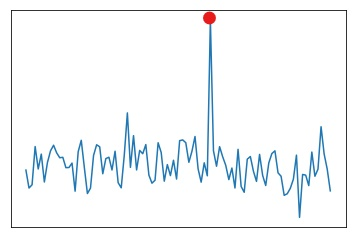
\includegraphics[height=6cm]{anomaly_point}
	\caption{Pointwise anomaly}
	\label{fig:point}
	\end{subfigure}
	~
	\begin {subfigure}[t]{8cm}
	\centering
	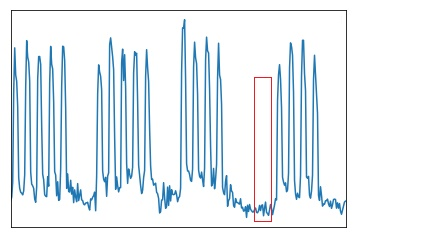
\includegraphics[ height=6cm]{anomaly_window}
	\caption{Window-based anomaly}
	\label{fig:window}
	\end{subfigure}
	\caption[Anomaly types]{Anomaly types}
\label{fig:anomalytypes}

\end{figure}


\section{LSTMs}
\label{sec:LSTMs}

Recurrent neural networks(RNNs) are widely used for speech, video recognition and prediction due to its recurrent property that captures the temporal dependency between data points in compare with other feed forward networks. However, the volume of RNN’s memory is limited, and vanishing gradient is also a difficulty by training RNNs. Therefore, the long short-term memory networks (LSTMs) are a kind of reinforced RNN that are able to remember valuable information in arbitrary time interval. A LSTM network is a recurrent neural network with neurons being LSTM units. \Fref{fig:lstmunit} shows a classical structure of a LSTM unit. LSTMs are able to capture long-term memory while there are a forget gate and a update gate in the LSTM unit, that select necessary previous information and new coming information according to the input data at each time step. The information is transferred to the next step along with the cell state. Besides, each LSTM units also output its value respectively.\\

\begin{figure}[ht]
\centering
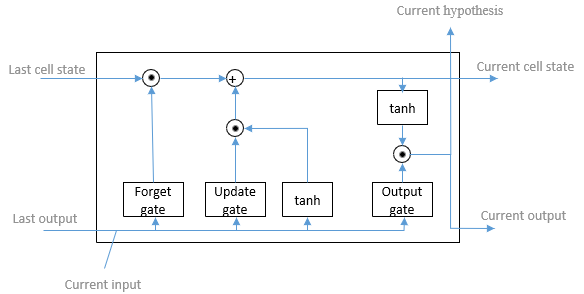
\includegraphics[width=12cm, height=8cm]{lstmunit}
\caption[LSTM unit]{The LSTM unit}
\label{fig:lstmunit}
\end{figure}


A LSTM unit can be unfolded over time, as shown in \Fref{fig:unfolded}. The LSTM unit takes a data window as input (one instance at each time step). Therefore, the LSTM unit extracts useful and drop useless temporal information from the window.\\


Deep LSTM RNNs are built by stacking multiple LSTM layers. Note that LSTM RNNs are already deep architectures in the sense that they can be considered as a feed-forward neural network unrolled in time where each layer shares the same model parameters. It has been argued that deep layers in RNNs allow the network to learn at different time scales over the input\cite{deep}. \Fref{fig:deeplstm} is a example of stacked deep LSTM neural network, there are 3 LSTM layers, each can be unfolded into 5 time steps, so the LSTMs take a window in length 5 as input and the output is in same size.\\

\begin{figure}[h]
\centering
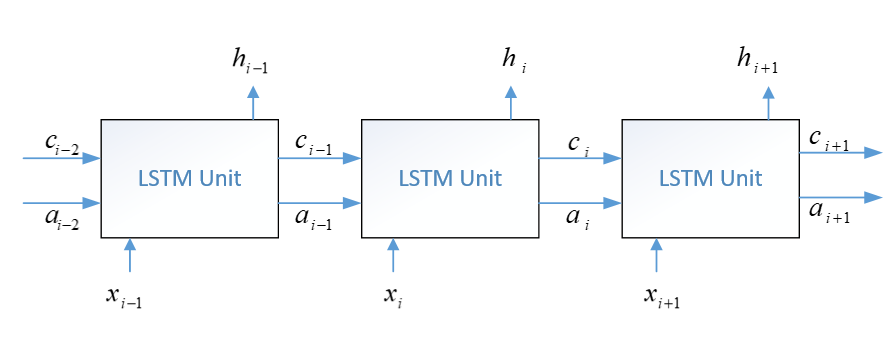
\includegraphics[width=12cm, height=5cm]{unfold}
\caption[Unfolded LSTM unit]{Unfolded LSTM unit}
\label{fig:unfolded}
\end{figure}

\begin{figure}[h]
\centering
	\begin {subfigure}[t]{0.45\textwidth}
	\centering
	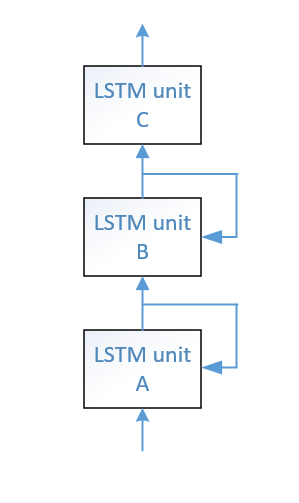
\includegraphics[height=6cm]{deepfolderedlstm}
	\caption{Deep folded LSTMs}
	\label{fig:deeplstm1}
	\end{subfigure}
	~
	\begin {subfigure}[t]{0.45\textwidth}
	\centering
	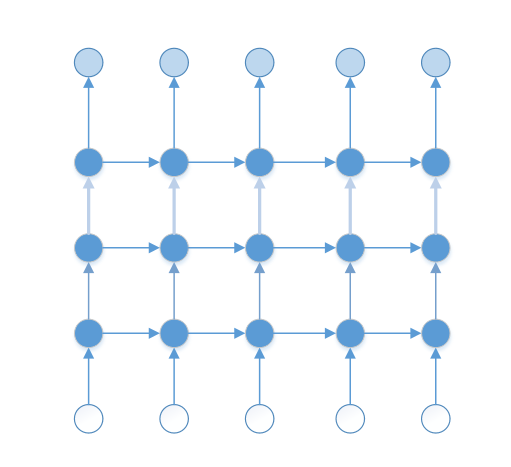
\includegraphics[ height=6cm]{deeplstm}
	\caption{Deep unfolded LSTMs. Each horizontal dark dot chain is an unfoldered LSTM unit over time, hollow dots and grey dots are windows of inputs and outputs.}
	\label{fig:deeplstm2}
	\end{subfigure}
	\caption[Deep LSTMs]{Deep LSTMs}
\label{fig:deeplstm}

\end{figure}

\section{Autoencoders}
\label{sec:Autoencoders}

An autoencoder (\Fref{fig:autoencoder}) is an artificial neural network with symmetrical structure. Normally an autoencoder has at least one hidden layer that consists of less neurons than input and output layers. And the basic aim of autoencoders is to reconstruct its own input and learn a lower dimensional representation (encoding) of input data in the hidden layer. Moreover, the autoencoders are also used for anomaly detection by measuring the reconstruction error between inputs and predictions.
Normally the component between input layer and hidden layer is called encoder, and the symmetrical component between hidden layer and output layer is called decoder. For input $\chi$, the objective function is to find weight vectors for encoder and decoder to minimize the reconstruction error (Equation \ref{eq:autoencoder}).\\

\begin{figure}[h]
\centering
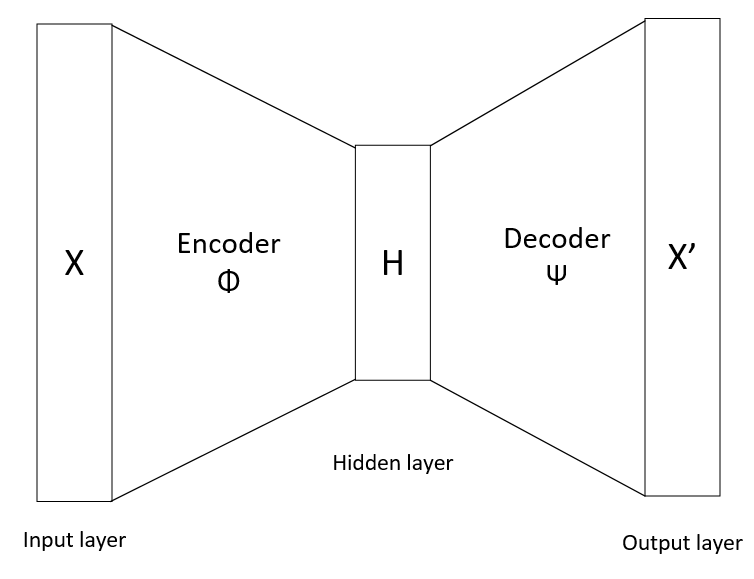
\includegraphics[width=7cm, height=5cm]{autoencoder}
\caption[Autoencoder]{Autoencoder}
\label{fig:autoencoder}
\end{figure}

\begin{equation} \label{eq:autoencoder}
\begin{aligned}
\Phi : &\chi \rightarrow H \\
\Psi : &H \rightarrow \chi \\
\Phi, \Psi = &argmin \left \| X-(\Psi \circ \Phi)X \right \|^2
\end{aligned}
\end{equation}

LSTMs-autoencoder has the same encoder-decoder architecture, while the neurons are LSTM units and connected in the way described in section \ref{sec:LSTMs}. \Fref{fig:encdecad} is a basic LSTMs-based autoencoder architecture with single LSTM layer on both encoder and decoder side. Our incremental LSTMs-autoencoder is based on this structure. The model takes window with length T as input (one instance at each step). The cell state carries sequence information and is passed through LSTM unit over time. When the encoder reaches the last encoder state, namely ET in \Fref{fig:encdecad2}, its cell state is actually the fix length embedding of the input window, and will be copied to the decoder as initial cell state of decoder, so that the input information is also transferred to the decoder. And the decoder predict the window in reversed order in order to make the optimization problem easier. To be notice that, different from aforementioned deep LSTMs in section \ref{sec:LSTMs}, the encoder outputs at each time step are not directly used as inputs of decoder, while between the encoder and decoder is actually not the same logical connection as stacked LSTMs. Here, the outputs of encoder are ignored, and there are different works contributes to the research of decoder inputs. Cho et al. \cite{phraserepresentation} feeds the input sequence to the decoder for a learning phrase representation task, Malhotra et al. \cite{encdecad} feed to decoder LSTM unit at each time step the value of previous time step as input, and in a extended work \cite{timenet} they feed the decoder always a constant vector for an anomaly detection task, because the finial cell state already carries all relevant information to represent the input window. In our model, we feed the decoder a constant vector.\\

\begin{figure}[t!]
\centering
	\begin {subfigure}[t]{0.45\textwidth}
	\centering
	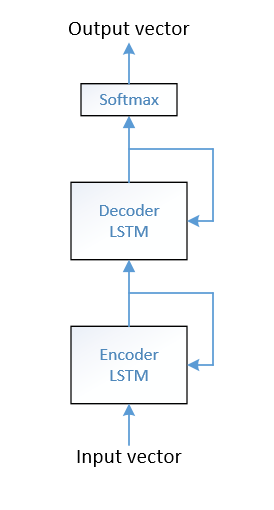
\includegraphics[height=6cm]{folded_encdecad}
	\caption{Folded LSTMs-Autoencoder}
	\label{fig:encdecad1}
	\end{subfigure}
	~
	\begin {subfigure}[t]{0.45\textwidth}
	\centering
	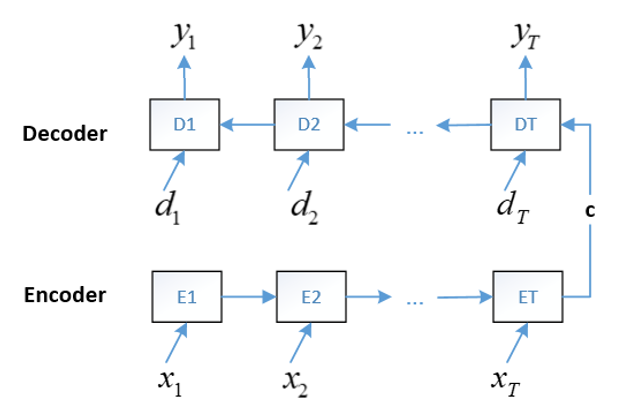
\includegraphics[ height=6cm]{encdecad2}
	\caption{Unfolded LSTMs-Autoencoder}
	\label{fig:encdecad2}
	\end{subfigure}
	\caption[LSTMs-Autoencoder]{LSTMs-Autoencoder}
\label{fig:encdecad}

\end{figure}






